%!TEX root = main.tex
\setcounter{chapter}{4}
\setcounter{section}{1}
\setcounter{theorem}{0}
\setcounter{equation}{0}

\lectureheader{161}{Calculus I}{Extreme value theorem}{\textit{Thomas' Calculus} \thesection}

\begin{definition}
Let $f$ be a function defined on the domain $D$.
\begin{itemize}
\item We say that $f$ attains a \textbf{global} (or \textbf{absolute}) \textbf{maximum on $D$} if there is a $c\in D$ so that $f(x)\le f(c)$ for all $x\in D$, in which case we say that $f(c)$ is the global (or absolute) maximum value of $f$ on $D$.
\item We say that $f$ attains a \textbf{global} (or \textbf{absolute}) \textbf{minimum on $D$} if there is a $c\in D$ so that $f(x)\ge f(c)$ for all $x\in D$, in which case we say that $f(c)$ is the global (or absolute) minimum value of $f$ on $D$.
\item Generically, we refer to global maximums and minimums as \textbf{global extrema} or \textbf{extreme values}.
\end{itemize}
\end{definition}
\begin{remark}
The global maximum/minimum is the value $y=f(c)$; the value $x=c$ is its location.
\begin{itemize} 
\item It is correct to say that $f$ has a global maximum/minimum of $y=f(c)$ at $x=c$.
\item It is wrong to say that $(c,f(c))$ is the global maximum/minimum.
\end{itemize}
\end{remark}
\vfill

\begin{remark}
Given function on a given domain, the global maximum/minimum may or may not exist.
If it does exist, there can be only one of each type.
\end{remark}
\begin{center}
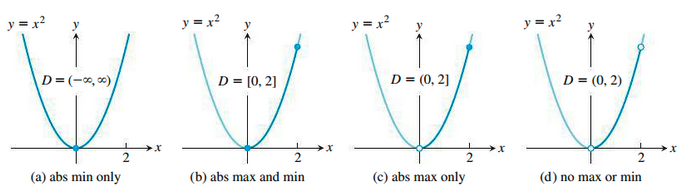
\includegraphics[width=6.5in]{img/nonexistence_of_extrema}
\end{center}
\vfill

\begin{theorem}[Extreme value theorem]
If $f$ is continuous on the closed, finite-length interval $[a,b]$, then $f$ attains both an global maximum and a global minimum on $[a,b]$.
\end{theorem}

\newpage

\begin{definition}
Let $f$ be a function defined on the domain $D$.
\begin{itemize}
\item We say that $f$ attains a \textbf{local} (or \textbf{relative}) \textbf{maximum on $D$} if there is a $c\in D$ and an $\epsilon>0$ so that $f(x)\le f(c)$ for all $x\in D\cap (c-\epsilon, c+\epsilon)$, 
in which case we say that $f(c)$ is the local (or relative) maximum value of $f$ on $D$.
\item We say that $f$ attains a \textbf{local} (or \textbf{relative}) \textbf{minimum on $D$} if there is a $c\in D$ and an $\epsilon>0$ so that $f(x)\ge f(c)$ for all $x\in D\cap (c-\epsilon, c+\epsilon)$, 
in which case we say that $f(c)$ is the local (or relative) minimum value of $f$ on $D$.
\item Generically, we refer to global maximums and minimums as \textbf{local extrema} or \textbf{extreme values}.
\end{itemize}
\end{definition}
\begin{remark}
The local maximum/minimum is the value $y=f(c)$; the value $x=c$ is its location.
\begin{itemize} 
\item It is correct to say that $f$ has a local maximum/minimum of $y=f(c)$ at $x=c$.
\item It is wrong to say that $(c,f(c))$ is the local maximum/minimum.
\end{itemize}
\end{remark}
\vfill

\begin{remark}\,
\begin{itemize}
\item A global maximum/minimum is always a local maximum/minimum, but not necessarily the reverse.
\item Each local maximum/minimum is a ``candidate" global maximum/minimum.
\end{itemize}
\end{remark}
\begin{center}
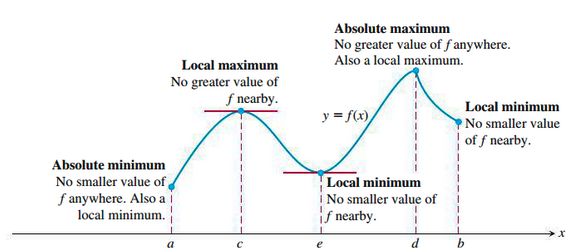
\includegraphics[width=6in]{img/global_vs_local_extrema}
\end{center}
\vfill

\newpage

\begin{theorem}
If $f$ has a local extremum at an interior point $x=c$ of its domain, then either $f'(c)=0$ or $f'(c)$ does not exist.
\end{theorem}
\begin{proof}\,

\vspace{6in}
\end{proof}

\vfill
\begin{definition}
An interior point of the domain of $f$ where $f'$ is zero or undefined is called a \textbf{critical point of $f$}.
\end{definition}
\begin{remark}
Critical points are ``candidate locations" for relative maxima/minima.
\end{remark}

\newpage

\begin{remark}[Optimization over compact intervals]\,\\
To find the global maximum/minimum of $y=f(x)$ over $[a,b]$:
\begin{enumerate}
\item Determine all critical points of $f$ in $(a,b)$.
\item Evaluate $f$ at all critical points as well as the endpoints $x=a$ and $x=b$.
\item The least $y$-value is the global minimum; the greatest $y$-value is the global maximum.
\end{enumerate}
\end{remark}
\begin{example}
Compute the global maximum and minimum of $f(x)=x^2$ over $[-2,1]$.
\end{example}
\vfill

\begin{example}
Compute the global maximum and minimum of $g(t)=8t-t^4$ over $[-2,1]$.
\end{example}
\vfill

\newpage

\begin{example}
Compute the global maximum and minimum of $f(x)=x^{2/3}$ over $[-2,3]$.
\end{example}
\vfill

\begin{example}
Suppose that at any given time $t$ (in seconds) the current $i$ (in amperes) in an alternating current circuit is
$i=2\cos t + 2\sin t$.
What is the peak (largest magnitude) current for this circuit?
\end{example}
\vfill

